\chapter{THE STATE OF THE ART AND THE INTEGRATION OF PLM AND MES} 
\pagenumbering{arabic} %設定頁號阿拉伯數字
\setcounter{page}{17}  %設定頁數
\begin{center}
\fontsize{18}{16}\selectfont \textbf{最先進的技術以及 PLM 和 MES 的集成}\\
\end{center}
\vspace{2em}

\fontsize{14pt}{2.5pt}\sectionef 
{Unfortunately, there are not many published studies in the matter of integration between PLM and MES systems. But there seems to be a consensus in the most probable effects of said integration. Those being synchronization and tighter tolerances.}\\[10pt]

\fontsize{14pt}{5pt}\sectionef
 {遺憾的是,關於 PLM 和 MES 系統整合問題的已發表研究並不多。但對於上述整合最可能產生的影響似乎已達成共識。這些是同步和更嚴格的公差。}\\[15pt]

\fontsize{14pt}{2.5pt}\sectionef 
{As explained by D’Antonio et al. (2015), which focus on a case study involving the manufacturing of precision components for aeronautical applications, the first advantage expected by the deployment of the monitoring and control system is product quality improvement: sensors allow to detect, measure and monitor variables, events and situations that affect process performance or product quality.}\\[10pt]

\fontsize{14pt}{5pt}\sectionef
 {正如德安東尼奧等人所解釋的。 (2015),重點在於涉及航空應用精密零件製造的案例研究,部署監控系統預期的第一個優勢是產品品質改進:感測器允許檢測、測量和監控變數、事件和影響製程性能或產品品質的情況。
}\\[15pt]

\fontsize{14pt}{2.5pt}\sectionef 
{One of the central problems regarding integrating PLM with any other system revolves around the ownership of information. A possible solution relies on database integration as well as the use of middleware between systems. As is written in Saaksvuori and Immonen, (2008). A reasonable objective is that information should always be updated in one place. Other systems can read information directly from the PLM databases, and if necessary, the required information can be replicated on the databases of other system, as depicted in Figure7. Although it points this out mainly from the perspective of PLM-ERP integration, it is still very valuable from the perspective of PLM-MES integration because it is an example of how the better operation can be expected by working around systems in which files of different nature are loaded into a centralized PLM-ERP system.}\\[10pt]

\fontsize{14pt}{5pt}\sectionef
 {將 PLM 與任何其他系統整合的核心問題之一涉及資訊的所有權。一種可能的解決方案依賴於資料庫整合以及系統之間中間件的使用。正如 Saaksvuori 和 Immonen (2008) 所寫。一個合理的目標是資訊應始終在一個地方更新。其他系統可以直接從PLM資料庫中讀取訊息,如果需要,可以將所需資訊複製到其他系統的資料庫上,如圖7所示。雖然主要是從PLM-ERP整合的角度指出了這一點,但從PLM-MES 整合的角度來看,仍然非常有價值,因為它是一個範例,說明如何透過將不同性質的檔案載入到集中式PLM-ERP 系統中的系統來實現更好的操作。
}\\[15pt]
\begin{figure}[hbt!]
\begin{center}
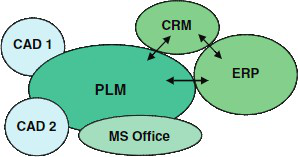
\includegraphics[width=10cm]{7}
\caption{\Large Diagram of PLM integration PLM整合示意圖}\label{fig.7}
\end{center}
\end{figure}

\fontsize{14pt}{2.5pt}\sectionef 
{The middleware would therefore be a software framework to organize and connect all the information given to the system database in a user-friendly way. This sort of application is also referred to as integration application and, as specified by Stark (2015), these applications enable exchange of product information between PLM applications (for example, between a CAD application and a CAE application). They also enable exchange of product information between PLM applications and other enterprise applications such as ERP and CRM.}\\[10pt]

\fontsize{14pt}{5pt}\sectionef
 {因此,中間件將成為一個軟體框架,以使用者友好的方式組織和連接提供給系統資料庫的所有資訊。此類應用程式也稱為整合應用程序,並且根據 Stark (2015) 的規定,這些應用程式支援在 PLM 應用程式之間(例如 CAD 應用程式和 CAE 應用程式之間)交換產品資訊。它們還支援 PLM 應用程式與其他企業應用程式(例如 ERP 和 CRM)之間的產品資訊交換。}\\[15pt]

\fontsize{14pt}{2.5pt}\sectionef 
{In a very relevant fashion, this middleware line of thinking is expanded upon by (Ben Khedher et al., 2011). In their work regarding different systems architectures for the implementation of an integrated MES+PLM they describe the use of a mediation system in web service architecture. As depicted in Figure 8, the proposed architecture uses data exchange based on internet technologies to help companies, especially expanded companies, to take advantage of opportunities generated by the Web Services. The concept of "web service" means an application (program or software system) which is designed to support interoperable machine-to-machine interactions over a network, according to the definition of W3C (Ben Khedher et al., 2011).}\\[10pt]

\fontsize{14pt}{5pt}\sectionef
 {(Ben Khedher et al., 2011) 以非常相關的方式擴展了這種中間件思路。在他們關於實施整合 MES+PLM 的不同系統架構的工作中,他們描述了中介系統在 Web 服務架構中的使用。如圖 8 所示,所提出的架構使用基於互聯網技術的資料交換來幫助公司,特別是擴張型公司,利用 Web 服務產生的機會。根據 W3C 的定義,「Web 服務」的概念是指旨在支援網路上可互通的機器對機器互動的應用程式(程式或軟體系統)(Ben Khedher 等,2011)。}\\[15pt]
\newpage

\begin{figure}[hbt!]
\begin{center}
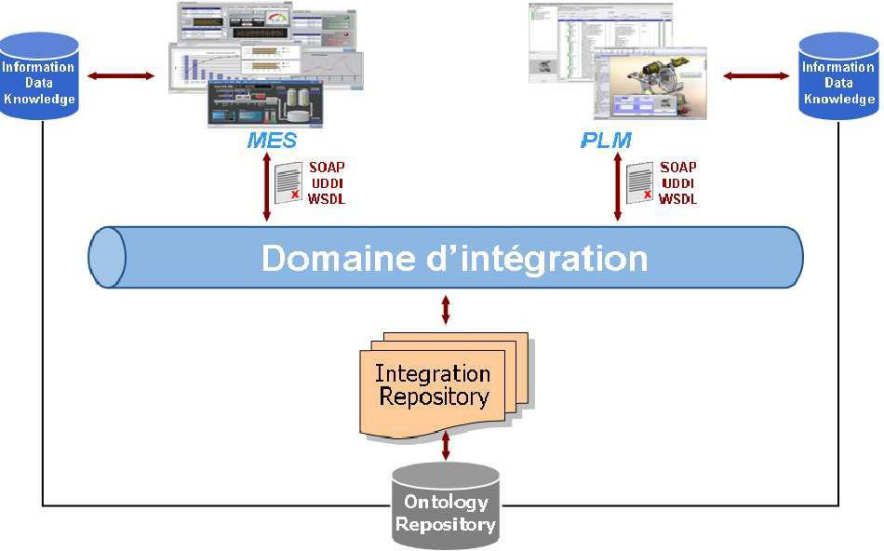
\includegraphics[width=15cm]{8}
\caption{\Large Diagram of Web service architecture Web服務架構圖}\label{fig.8}
\end{center}
\end{figure}

\fontsize{14pt}{2.5pt}\sectionef 
{The reason this expansion is so relevant from the perspective of this work is that the Odoo software works in a similar fashion through a similar web service architecture. In theory the Odoo software could act as the middleware working through the local network or hosted in the cloud and enacting the layer of integration that was previously mentioned.}\\[10pt]

\fontsize{14pt}{5pt}\sectionef
 {從這項工作的角度來看,這種擴展如此相關的原因是 Odoo 軟體透過類似的 Web 服務架構以類似的方式運作。理論上,Odoo 軟體可以充當透過本地網路工作或託管在雲端中的中間件,並執行前面提到的整合層。}\\[15pt]

\section{How would this integration look like in practical terms 這種整合在實際中會是什麼樣子}

\fontsize{14pt}{2.5pt}\sectionef 
{As mentioned in CHAPTER 2 the main idea of PLM is to manage change in all processes related to the product, and it does so mainly through the use of virtualization. The word virtualization here denotes representation of item of the real world to the digital space and, as one can imagine, there are several levels of abstraction through which a real object or process can be represented. As consequence there is no exact consensus regarding PLM of how deep and/or detailed the virtual representation must be to serve its purpose.}\\[10pt]

\fontsize{14pt}{5pt}\sectionef
 {如第 2 章中所提到的,PLM 的主要想法是管理與產品相關的所有流程中的變更,它主要透過使用虛擬化來實現。這裡的「虛擬化」一詞表示現實世界的項目在數位空間中的表示,並且正如人們可以想像的那樣,可以透過多個抽象層級來表示真實的物件或過程。因此,對於 PLM 虛擬表示必須有多深和/或多詳細才能達到其目的,還沒有達成確切的共識。}\\[15pt]

\fontsize{14pt}{2.5pt}\sectionef 
{In an ideal world that would be the lowest form of abstraction which, essentially, would come down to a digital twin as explained in the CHAPTER 2. This is a ‘1 to 1’ digital representation of every aspect of the production cycle where every part involved would have a digital representation that not only carry the physical characteristics of the item but also all its information produced over time. To this end, as explained in CHAPTER 2, MES takes a fundamental role in obtaining the real time information required for the DT even be possible.}\\[10pt]

\fontsize{14pt}{5pt}\sectionef
 {在理想的世界中,這將是最低的抽象形式,本質上將歸結為數位孿生,如第 2 章所述。這是生產週期各個方面的「1 對 1」數字表示,其中每個部分所涉及的內容將具有數位表示,不僅包含該項目的物理特徵,還包含隨著時間的推移產生的所有資訊。為此,如第 2 章所述,MES 在獲取 DT 所需的即時資訊方面發揮基礎作用,甚至是可能的。}\\[15pt]

\fontsize{14pt}{2.5pt}\sectionef 
{For instance, a CNC machine would have a digital 3D model for simulation as well as a fully integrated list of all the pieces it produces, data regarding its current level of production, the current wear of its mechanical pieces, all other machines it relates to, history of all the alterations and improvements by which it was affected and many other aspects, all well packaged in an intuitive graphical user interface (GUI) that allows for maximum interaction.}\\[10pt]

\fontsize{14pt}{5pt}\sectionef
 {例如,數控機床將具有用於模擬的數位 3D 模型以及其生產的所有零件的完全整合清單、有關其當前生產水平的數據、其機械零件的當前磨損情況以及與其相關的所有其他機器、受影響的所有變更和改進的歷史記錄以及許多其他方面,全部都很好地封裝在直覺的圖形使用者介面(GUI) 中,可實現最大程度的互動。}\\[15pt]

\fontsize{14pt}{2.5pt}\sectionef 
{Outside of fiction, we are yet to achieve such level of virtualization. It takes too much time and money to obtain and organize information to such a level of minutia, specially, the aspects that need to be inserted by hand, not to mention the subjectiveness of how this information can be integrated and interacted with. Regardless of that it is useful to identify, within the ideal, the aspects of most importance for this implementation.}\\[10pt]

\fontsize{14pt}{5pt}\sectionef
 {除了小說之外,我們還沒有達到這樣的虛擬化程度。獲取和組織如此詳細的資訊需要花費太多的時間和金錢,特別是需要手動插入的方面,更不用說如何整合和互動這些資訊的主觀性了。不管怎樣,在理想情況下確定對於此實施最重要的方面是有用的。}\\[15pt]

\fontsize{12}{2.5pt}\selectfont {Those are:}\\[1pt]
\fontsize{12}{2.5pt}\selectfont {那些是:}\\[15pt]

\begin{enumerate}[{\hspace{0.5em}\textbullet}]
\fontsize{12}{2.5pt}\selectfont
\item The means of virtualization – What sort of information is used to build the virtual items. This includes the metadata and files that are directly attached to the item. In an ideal fashion this would contain all possible information available about the item.\\
虛擬化的手段-使用什麼樣的資訊來建構虛擬物品。這包括直接附加到項目的元資料和文件。在理想的情況下,這將包含有關該項目的所有可能的可用資訊。
\item The means of data input - How this information is being loaded and organized. Ideally this information would be loaded into the system as automatically as possible, be it by means of MES during quality control or through the use of automated input tools like bar code scanners.\\
資料輸入的方式 - 如何載入和組織這些資訊。理想情況下,這些資訊將盡可能自動載入到系統中,無論是在品質控制期間透過 MES 還是透過使用條碼掃描器等自動輸入工具。
\item The means of access – How this information is presented to the users. Although more subjective than the previous aspects this is incredibly important to the way the system is interacted with. How intuitive it is the information availability plays right into the core strengths of PLM. Afterall, everything would be for nothing (even if all else would be perfect) if the only way to interact with the system were a command line interface that would make difficult for the end users to access the information.\\
存取方式-如何將資訊呈現給使用者。儘管比前面的方面更主觀,但這對於系統互動的方式非常重要。資訊可用性的直覺程度正是 PLM 的核心優勢。畢竟,如果與系統互動的唯一方式是命令列介面,而這將使最終用戶存取資訊變得困難,那麼一切都將毫無意義(即使其他一切都很完美)。
\item The means of integration - How items and their contained information can interact and benefit from one another, i.e., the integration with other systems and key softwares. E.g., if an item has access to a cad file, there should be no need to fill in the metadata fields by hand. Hoe items can automatically affect other items also plays into this aspect.\\
整合方式 - 專案及其所包含的資訊如何互動並相互受益,即與其他系統和關鍵軟體的整合。例如,如果某個項目可以存取 cad 文件,則無需手動填寫元資料欄位。鋤頭項目可以自動影響其他項目也能發揮作用。

\end{enumerate}
\renewcommand{\baselinestretch}{0.5} %設定行距